\subsection{Model Scotta \(D_\infty\)}
W rozdziale tym przybliżymy konstrukcję modelu Scotta \(D_\infty\) zgodnie z \cite[Rozdział 16]{Hindley:2008:LCI:1388400}. Ze względu na obszerność materiału zaprezentujemy wyłącznie konstrukcję modelu bezsyntaktycznego (ang. \emph{syntax-free}) przemilczając jego topologiczny charakter. %i topologiczny charakter modelu szczegółowe wyprowadzenia będą elementarne lub zostaną pominięte.

\paragraph{Wprowadzenie}
Ustalmy wpierw, że nie możemy naiwnie interpretować \(\lambda\)-termów jako funkcji i aplikacji argumentów do funkcji. Przypuśćmy bowiem, że w pewnej interpretacji \(\llbracket M \rrbracket=f_M\), gdzie \(f_M \in A\to B\) dla pewnych zbiorów \(A\) i \(B\). Wówczas \(\llbracket M M\rrbracket=\nobreak f_M(f_M)\), a zatem \(f_M\in A\). Oznacza to, że funkcja \(f_M\) jest elementem swojej własnej dziedziny i możliwe jest skonstruowanie nieskończonego zstępującego ciąg zbiorów:
\[
  f_M \ni (f_M, f_M f_M)  \ni\{f_M\} \ni f_M \ni \dots
\]
Istnienie takiego ciągu narusza jednak aksjomat ufundowania na gruncie aksjomatyki ZF, a to wyklucza możliwość określenia takich modeli.

Rozwiązanie Scotta polega na tym, aby zamiast próbować interpretować termy jako funkcje, przypisać im nieskończone ciągi funkcji postaci 
\[
  \varphi = (\varphi_0,\,\varphi_1,\,\varphi_2,\,\dots),
\]
gdzie \(\varphi \in D_\infty\) i \(\varphi_n\in D_n\). Określając na takiej strukturze aplikację następująco
\[
  \varphi\bullet\psi = (\varphi_1(\psi_0),\,\varphi_2(\psi_1),\,\varphi_3(\psi_2),\,\dots),
\]
widzimy, że samoaplikacja jest poprawnie określona: 
\[
  \varphi\bullet\varphi = (\varphi_1(\varphi_0),\,\varphi_2(\varphi_1),\,\varphi_3(\varphi_2),\,\dots).
\]

%\subsubsection{Wprowadzenie}
Celem wprowadzenia ustalmy szereg następujących pojęć.

\begin{definicja}[Struktura aplikatywna]
Parę \((D,\, \bullet)\), gdzie \(D\) jest zbiorem zawierającym przynajmniej dwa elementy i w którym symbol \(\bullet\) oznacza działanie binarne na \(D\), nazywamy \emph{strukturą aplikatywną}.
\end{definicja}
\begin{konwencja*}
  Ponieważ nie zakładamy, że działanie \(\bullet\) jest łączne, to celem ograniczenia ilości nawiasów przyjmijmy, że \(\bullet\) wiąże lewostronnie, czyli \(a\bullet b\bullet c\bullet d \equiv \left(\left(a\bullet b\right)\bullet c\right)\bullet d\).
\begin{definicja}[Ekstensjonala równoważność]%3.4
Niech \((D,\,\bullet)\) będzie strukturą aplikatywną i niech \(a,\,b\in D\). Określamy relację: 
\begin{align*}
a \sim b \quad \Leftrightarrow\quad \forall d \in D \left(a \bullet d = b \bullet d\right).
\end{align*}
Powiemy, że \(a\) jest \emph{ekstensjonalnie równoważne} \(b\), jeśli \(a\sim b\).
\end{definicja}

\end{konwencja*}
% Ustalmy teraz co rozumiemy przez \(\lambda\)-model.

% \begin{definicja}[Model syntaktyczny]%3.3
%   Trójkę \((D,\,\bullet,\,\llbracket\,\rrbracket)\), gdzie \((D,\,\bullet)\) jest strukturą aplikatywną, \(\llbracket\,\rrbracket_\rho\) jest funkcją przyporządkowującą elementy 
%   \(\llbracket M\rrbracket \in D\) termowi \(M\) przy wartościowaniu \(\rho\) (\emph{interpretacją} względem \(\rho\)), nazywamy \emph{\(\lambda\)-modelem}, jeśli spełnia poniższe własności:
%   \begin{enumerate}
%     \item \(\forall x \in V\ \left(\llbracket x \rrbracket_\rho = \rho(x)\right)\).
%     \item \(\forall M,\,N \in \mathbf{\Lambda}\ (\llbracket MN \rrbracket_\rho = \llbracket M\rrbracket_\rho \bullet \llbracket N \rrbracket_\rho)\).
%     \item \(\forall x \in V\,\forall M\in \mathbf{\Lambda}\,\forall d\in D\ (\, \llbracket \lambda x.\,M\rrbracket_\rho \bullet d = \llbracket M \rrbracket_{\rho[x/d]})\).
%     \item Dla dowolnych wartościowań \(\rho\),  \(\sigma\) i dowolnego termu \(M\in\nobreak\mathbf{\Lambda}\), jeśli \[\forall x\in\nobreak\mathrm{FV}(M)\ (\rho(x) =\nobreak \sigma(x)),\] to \(\llbracket M\rrbracket_\rho =\nobreak\llbracket M \rrbracket_\sigma\).
%     \item \(\forall M\in\mathbf{\Lambda}\,\forall x, y\in V\ (y\not\in\mathrm{FV}(M)\implies \llbracket\lambda x.\,M\rrbracket_\rho = \llbracket \lambda y.\,M[x/y]\rrbracket_\rho) \).
% %    \item \(\forall M,\,N\in\mathbf{\Lambda}\,\left(\forall d\in D\,(\llbracket M\rrbracket_{\rho[x/d]}=\llbracket N \rrbracket_{\rho[x/d]} ) \implies \llbracket \lambda x.\,M\rrbracket_\rho = \llbracket \lambda x.\,N\rrbracket_\rho\right)\).
%     \item \(\forall M,\,N\in\mathbf{\Lambda}\,\left(\llbracket\lambda x.\,M\rrbracket_\rho \sim \llbracket \lambda x.\,N\rrbracket_\rho\ \implies \llbracket \lambda x.\,M\rrbracket_\rho = \llbracket \lambda x.\,N\rrbracket_\rho\right)\).
%   \end{enumerate}
% \end{definicja}

% Żądamy przede wszystkim, aby interpretacja \(\lambda\)-termów była zachowawcza ze względu na \(\beta\)-konwersję: chcemy utożsamiać ze sobą interpretacje \(\beta\)-konwersów tak aby ich znaczeniem była postać normalna (lub jej brak). Aplikacja jest w istocie działaniem binarnym na termach. Dlatego na uniwersum interpretacji wprowadzamy działanie \(\bullet\) tak, aby \(\llbracket M\rrbracket_\rho \bullet \llbracket N \rrbracket_\rho = \llbracket MN \rrbracket_\rho\) (Warunek 2). Warunek 3 jest konsekwencją obserwacji, że \((\lambda x.\,M) N =_\beta M[x/N]\), a zatem oczekujemy, aby 
% \[
%   \llbracket \lambda x.\,M \rrbracket_\rho \bullet \llbracket N \rrbracket_\rho =
%   \llbracket (\lambda x.\,M) N\rrbracket_\rho = \llbracket M[x/N \rrbracket_\rho.
% \]
% Interpretacja rezultatu operacji podstawienia termu \(N\) za zmienną \(x\) nie różni się jednak w tym wypadku niczym od zmiany wartościowania zmiennej \(x\) przez interpretację termu \(\llbracket N\rrbracket_\rho\) (symbolicznie: \(\rho[x/\llbracket N \rrbracket_\rho])\), bowiem w wyniku \(\beta\)-redukcji żadna nowa zmienna nie zostaje związana i zastąpione przez \(N\) zostają wszystkie wolne wystąpienia \(x\) w \(M\). Waruneki 4 i 5 odpowiadają utożsamieniu \(\alpha\)-konwersów.


\begin{definicja}% kombinacja zmiennycha, 3.7
\begin{enumerate}
  \setlength\itemsep{0em}
\item
Powiemy, że term \(M\) jest \emph{kombinacją zmiennych}, jeśli \(M\equiv x\) dla pewnej zmiennej \(x\) albo \(M\equiv (PQ)\) dla pewnych kombinacji zmiennych \(P\) i \(Q\). 
\item 
Niech \(M\) będzie kombinacją zmiennych taką, że \(\mathrm{FV}(M)=\{x_1,\,x_2,\,\dots,\,x_n\}\). Względem \(M\) określamy funkcję \(f_M: D^n\to D\) następującym wzorem:

% \begin{align*}
% f_M (d_1,\,d_2,\,\dots,\,d_n) = \begin{cases}
% d_k,\ \text{jeśli}\ M\equiv x_k \text{dla pewnego}\ 1\leq k \leq n,\\
% f_Q (d_1,\,d_2,\,\dots,\,d_n) \bullet f_Q (d_1,\,d_2,\,\dots,\,d_n)\  \text{jeśli}\ M\equiv (QR)\ \text{dla pewnych kombinacji zmiennych QR}.
% \end{cases}
% \end{align*}
\begin{align*}
f_M (d_1,\,d_2,\,\dots,\,d_n) = \begin{cases}
d_k,\ &\text{jeśli}\ M\equiv x_k, \\
f_P (d_1,\,d_2,\,\dots,\,d_n) \bullet f_Q (d_1,\,d_2,\,\dots,\,d_n),\ & \text{jeśli}\ M\equiv (PQ).
\end{cases}
\end{align*}

\item
Powiemy, że struktura aplikatywna \((D,\,\bullet)\) jest \emph{kombinatorowo zupelna}, jeśli dla każdej kombinacji zmiennych \(M\) istnieje \(a_M\in D\) taki, że dla wszystkich \(d_1\),\(d_2\),\(\dots\),\(d_n\in D\)
\[
  a_M\bullet d_1 \bullet d_2 \bullet \dots \bullet d_n = f_M(d_1,\, d_2,\,\dots,\,d_n).
\]
\end{enumerate}
\end{definicja}


\begin{definicja}[Model bezsyntaktyczny]%3.9
  Modelem bezsyntaktycznym rachunku \(\lambda\) nazywamy trójkę \((D,\,\bullet, \Lambda)\), gdzie \(\mathbb{D}=(D,\,\bullet)\) jest strukturą aplikatywną, \(\Lambda: D \to D\) i spełnione są poniższe własności:
  \begin{enumerate}[label={(\alph*)}, ref={(\alph*)}]
  \setlength\itemsep{0em}
    \item \(\mathbb{D}\) jest kombinatorowo zupełny.
    \item \(\Lambda (a) \sim a\) dla wszystkich \(a\in D\).
    \item Jeśli \(a\sim b\), to \(\Lambda(a) = \Lambda(b)\) dla wszystkich \(a,\,b\in D\).
    \item \(\Lambda(a)=e\bullet a\) dla pewnego \(e\in D\) i wszystkich \(a\in D\).
  \end{enumerate}
\end{definicja}

\paragraph{Elementy teorii porządku} 
Niech \((D,\sqsubseteq)\) będzie zbiorem częściowo uporzadkowanym. Powiemy, że \(b\in D\) jest elementem \emph{najmniejszym}, jeśli \(b\sqsubseteq d\) dla wszystkich \(d\in D\). Element ten, o ile istnieje, wyznaczony jest jednoznacznie i będziemy oznaczać go symbolem \(\perp\). Niech \(X\subset D\). \emph{Ograniczeniem górnym} \(X\) nazywamy element \(u\in D\) taki, że \(x\sqsubseteq u\) dla wszystkich \(x\in X\). \emph{Kresem górny} zbioru \(X\) nazywamy element \(\ell\in D\) taki, że \(\ell\) jest ograniczeniem górnym \(X\) i \(\ell\sqsubseteq u\) dla wszystkich ograniczeń górnych \(u\) zbioru \(X\). Element taki, o ile istnieje, będziemy oznaczali symbolem \(\bigsqcup X\). Podzbiór \(X\subset D\) nazywamy \emph{skierowanym}, jeśli \(X\neq\emptyset\) i dla dowolnych \(x, y\in X\) istnieje \(z\in X\) taki, że \(x\sqsubseteq z\) i \(y\sqsubseteq z\). 

\begin{definicja}[Zupełny porządek częściowy]%5.1
Porządek częściowy \((D,\,\sqsubseteq)\) taki, że
\begin{enumerate}[label={(\alph*)}, ref={(\alph*)}]
  \setlength\itemsep{0em}
  \item posiada element najmniejszy oraz
  \item każdy skierowany poddzbiór \(X\subset D\) ma kres górny,
\end{enumerate}
  nazywamy \emph{zupełnym porządkiem częściowym} (w skrócie: \emph{cpo}).
\end{definicja}

Ustalmy, że jeśli \(D'\), \(D''\), \(\dots\)  są cpo, to odpowiadające im porządki częściowe będziemy notowali symbolami \(\sqsubseteq'\), \(\sqsubseteq''\), \(\dots\)

\begin{przyklad}\label{ex:scott_d0}
  Ustalmy \(\perp\not\in \mathbb{N}\) i niech \(\mathbb{N}^{+}=\mathbb{N}\cup{\perp}\). Określmy na \(\mathbb{N}^+\) następującą relację:
  \begin{align*}
    a \sqsubseteq b \quad \Leftrightarrow\quad (a=\perp\ \land\ b\in \mathbb{N})\ \lor\ a = b
  \end{align*}
  \(\sqsubseteq\) jest oczywiście zwrotna, przechodnia i antysymetryczna. Widzimy, że \(\mathbb{N}^{+}\) ma względem niej element najmniejszy (jest nim  \(\perp\)). Podzbiory jednoelementowe \(\mathbb{N}^{+}\) i podzbiory dwuelementowe zawierające \(\perp\) to wszystkie skierowane podzbiory \(\mathbb{N}^{+}\). Widzimy, że każdy z nich ma kres górny, a zatem \(\mathbb{N}^{+}\) jest cpo.
\end{przyklad}

\begin{definicja}[Monotoniczność, ciągłość, ścisłość]\label{def:m_cont}%5.3
Niech \(D\) i \(D'\) bedą cpo i \(\varphi: D\to D'\).
\begin{enumerate}[label={(\alph*)}, ref={(\alph*)}] 
  \setlength\itemsep{0em}
\item Powiemy, że \(\varphi\) jest \emph{monotoniczna}, jeśli \(\varphi(a) \sqsubseteq' \varphi(b)\) dla \(a\sqsubseteq b\).
\item Powiemy, że \(\varphi\) jest \emph{ciągła (w sensie Scotta}\footnote{Funkcje te są ciągłe w topologicznym sensie względem topologii Scotta.}), jeśli \(\varphi(\bigsqcup X) = \bigsqcup \varphi (X)\) dla wszystkich skierowanych podzbioru \(X\subseteq D\).\label{def:m_cont_2}
\item Powiemy, że \(\varphi\) jest \emph{ścisła} (ang. \emph{strict}), jeśli \(\varphi(\perp)=\perp'\). Funkcje, które nie są ścisłe, nazywamy niekiedy \emph{leniwymi} (ang. \emph{lazy}).
\end{enumerate}
Symbolem \([D\to D']\) oznaczamy zbiór wszystkich funkcji ciągłych ze zbioru \(D\)~do~\(D'\).
\end{definicja}

\begin{uwaga*}
Zauważmy, że jeśli \(\varphi\) jest ciągła, to jest również monotoniczna. Istotnie, jeśli \(a\sqsubseteq b\), to w szczególności \(\{a, b\}\subseteq D\) jest skierowanym podzbiorem \(D\). Wówczas \(\bigsqcup\{a, b\}=b\) i ponieważ \(\bigsqcup \varphi(\{a\,b\})=\varphi(\bigsqcup\{a,\,b\})\), to otrzymujemy, że \(\varphi(a)\sqsubseteq \varphi(\bigsqcup\{a,\,b\}) = \varphi(b)\).
\end{uwaga*}

\begin{twierdzenie}%5.4
Jeśli \(D\) i \(D'\) są cpo, to \([D\to D']\) jest cpo.
  % \begin{enumerate}[label={(\roman*)}, ref={(\roman*)}]
  % \setlength\itemsep{0em}
    % \item \(([D\to D'], \preceq)\) jest cpo.
    % \item \(([D\to D'], \preceq)\) ma element najmniejszy.
    % \item Każdy skierowany podzbiór \(\Phi \in [D\to D']\) ma supremum.
     % \item \([D\to D']\) jest cpo.
     % \item \([D\to D']\) ma element najmniejszy.
     % \item Każdy skierowany podzbiór \(\Phi \in [D\to D']\) ma kres górny.
  % \end{enumerate} 
\end{twierdzenie}
\begin{dowod}
  % \begin{enumerate}[label={(\roman*)}, ref={(\roman*)}]
  % \setlength\itemsep{0em}
  %   \item 
      Określmy na \([D\to D']\) relację  \(\preceq\):
\[
\varphi \preceq \psi\quad \Leftrightarrow\quad \forall d\in D \left(\varphi(d) \sqsubseteq' \psi(d)\right),
\]
Ponieważ \(D'\) jest cpo, to aby wykazać, że \([D\to D']\) ma element najmniejszy, wystarczy, że rozpatrzymy \(\perp(d)=\perp'\) dla \(d\in D\).

Niech teraz \(\Phi\) będzie skierowanym podzbiorem \([D\to D']\). 
      Wówczas  dla  wszystkich  \(d\in D\)  zbiór  \(\{\varphi(d)\  |\ \varphi\in\Phi\}\) jest  skierowanym podzbiorem  \(D'\). Wybierzmy \(y_1,\,y_2\in\{\varphi(d)\ |\ \varphi\in\Phi\}\). Wówczas dla pewnych \(\varphi_1, \varphi_2\in\Phi\) mamy, że \(y_1=\varphi_1(d)\) oraz \(y_2=\varphi_2(d)\). Ponieważ \(\Phi\) jest skierowany, to istnieje \(\varphi_3\) taki, że \(\varphi_1\preceq \varphi_3\) i \(\varphi_2\preceq \varphi_3\). Wówczas dla dowolnego \(d\in D\) \(\varphi_1(d) \sqsubseteq' \varphi_3(d)\) oraz \(\varphi_1(d) \sqsubseteq' \varphi_3(d)\), a zatem zbiór \(\{\varphi(d)\  |\ \varphi\in\Phi\}\) istotnie jest skierowany dla każdego \(d\in D\). Ponieważ zaś \(D'\) jest cpo, to dla każdego \(d\in D\) istnieje kres górny  \(\{\varphi(d)\  |\ \varphi\in\Phi\}\). Określmy więc funkcję \(\Psi_\Phi: D\to D'\) następującym wzorem:
      \begin{align*}
        \Psi_\Phi(d) = \bigsqcup \Phi d,
      \end{align*}
      gdzie \(\Phi d=\{\varphi(d)\ |\ \varphi \in \Phi\}\). Wystarczy teraz pokazać, że \(\Psi_\Phi\) jest ciągla i jest kresem górnym zbioru \(\Phi\).
      \begin{enumerate}
        \item Pokażemy najpierw, że \(\Psi_\Phi\) jest ciągła. Niech \(X\) będzie dowolnym skierowanym podzbiorem \(D\). Wówczas:
          \begin{align*}
  \Psi_\Phi(\bigsqcup X)&= \bigsqcup \Phi (\bigsqcup X)\\
                        &= \bigsqcup \{\varphi(\bigsqcup X)\ |\ \varphi\in\Phi\}\\
                        &= \bigsqcup \left\{\bigsqcup\left\{\varphi(d)\ |\ d\in X\right\}\ |\ \varphi\in \Phi\right\}\\
                        &= \bigsqcup \left\{\bigcup\limits_{\varphi\in\Phi}\{\varphi(d)\ |\ d\in X\}\right\}\\
                        &= \bigsqcup \left\{\bigcup\limits_{\varphi\in\Phi}\bigcup\limits_{d\in X}\{\varphi(d)\}\right\}
                         =\bigsqcup \left\{\bigcup\limits_{d\in X}\bigcup\limits_{\varphi\in\Phi}\{\varphi(d)\}\right\}\\
                        &= \bigsqcup \left\{\bigcup\limits_{d\in X}\{\varphi(d)\ |\ \varphi\in\Phi \}\right\}\\
                        &= \bigsqcup \left\{\bigsqcup \{\varphi(d)\ |\ \varphi\in\Phi \}\ |\ d\in X\right\}\\
                        &= \bigsqcup \left\{\bigsqcup \Phi d\ |\ d\in X\right\}
                        = \bigsqcup \Psi_\Phi(X).
          \end{align*}
        \item Niech \(\varphi\in\Phi\). Wówczas dla dowolnego \(d\in D\) mamy \(\varphi(d)\sqsubseteq' \bigsqcup \Phi d = \Psi_{\Phi} d\). Zatem \(\varphi\preceq\Psi_\Phi\) i \(\Psi_\Phi\) jest ograniczeniem górnym \(\Phi\). Jeśli \(\Psi_\Phi\) nie jest kresem górnym \(\Phi\), to istnieje \(\chi\) takie, że \(\chi\preceq\Psi_\Phi\) oraz \(\chi\) jest kresem górnym \(\Phi\). Wówczas dla dowolnego \(d\in D\) mamy, że \(\chi(d)\) jest kresem górnym \(\Phi d\) oraz \(\chi(d)\sqsubseteq'\Psi_\Phi(d)\). Ale \(\Psi_\Phi(d)=\bigsqcup\Phi d\), a zatem \(\chi(d)\) nie jest kresem górnym \(\Phi d\). Stąd \(\Psi_\Phi\) jest kresem górnym \(\Phi\).   
        % \item \(\Phi\) jest ograniczony w \([D\to D']\). Istotnie, przypuśćmy, że dla dowolnego \(f\in[D\to D']\) istnieje \(g\in\Phi\) taki, że \(f\preceq g\). Wówczas w szczególności \(\Psi_\Phi \preceq g\) i stąd również
        %   \[
        %     \bigsqcup \Phi d \subseteq' g(d)\quad \text{dla wszystkich}\ d\in D.
        %   \]
        %   Ponieważ \(g\in\Phi\), to \(g(d)\subseteq \bigsqcup\{g(d)\ |\ g\in\Phi\}=\bigsqcup\Phi d\). Zatem \(\Psi_\Phi\) jest ograniczeniem górnym \(\Phi\).

        %   Przypuśćmy teraz, że \(\Phi\) nie ma kresu górnego. Wówczas dla dowolnego ograniczenia górnego \(f\) zbioru \(\Phi\) istnieje \(g\) takie, że \(g\preceq f\) i które jest również ograniczeniem górnym. Wówczas w szczególności mamy, że \(g\preceq \Psi_\Phi\), czyli dla dowolnego \(d\in D\)
        %   \[
        %     g(d) \subseteq' \bigsqcup \Phi  d\in D'.
        %   \]
        %   Ale \(\bigsqcup \Phi d\) jest kresem górnym \(\Phi d\) (wykazaliśmy bowiem, że \(\Phi d\) jest skierowany, zaś \(D'\) jest cpo), a zatem \(g(d)\) nie może być ograniczeniem \(\Phi d\). Istnieje stąd \(z\in \Phi d\) taki, że \(g(d)\subseteq' z\). Wówczas istnieje \(\tilde\varphi\in\Phi\) taki, że \(z=\tilde\varphi(d)\) oraz \(g(d)\subseteq' \tilde\varphi(d)\). Z dowolności \(d\) mamy, że \(g\preceq \tilde\varphi\). Zatem \(g\) nie jest ograniczeniem górnym \(\Phi\), co jest sprzeczne z założeniem. Stąd \(\Psi_\Phi\) musi być kresem górnym \(\Phi\).\qed
      \end{enumerate}
\end{dowod}
  \begin{definicja}\label{thm:scott_seq}
    Dla danego cpo \(D_0\) możemy skonstruować ciąg cpo \(\{D_n\}_{n=0}^{\infty}\) określając \(D_{n+1}=[D_n\to D_n]\) dla \(n\geq 0\). Tak określony ciąg dla \(D_0=\mathbb{N}^{+}\) (patrz Przykład \ref{ex:scott_d0}) nazywamy modelem Scotta.
  \end{definicja}
\begin{definicja}[Projekcja]%5.5
Niech \(D\) i \(D'\) będą cpo. \emph{Projekcją} z \(D'\) do \(D\) nazywamy parę \((\varphi, \psi)\) funkcji \(\varphi \in [D\to D']\), \(\psi \in [D'\to D]\) takich, że
\begin{align}
\psi\circ \varphi = I_D\quad \text{oraz}\quad \varphi\circ \psi \preceq I_{D'} %\tag{\textasteriskcentered},
\end{align}
gdzie przez \(I_D\) i \(I_{D'}\) oznaczamy funkcję identycznościową na zbiorze \(D\) i \(D'\), odpowiednio.
\end{definicja}

\begin{figure}[h]
  \centering
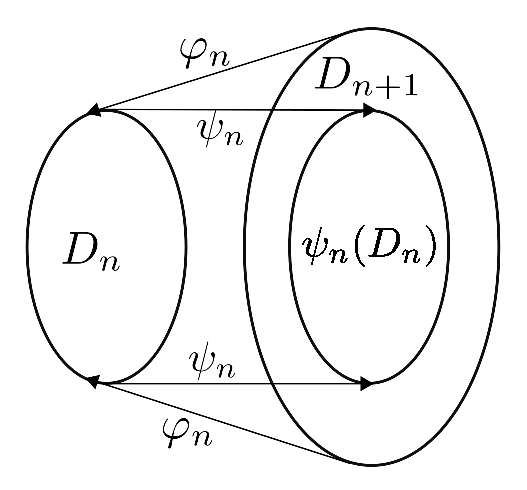
\includegraphics[width=0.32\linewidth]{../embeding_i}
  \caption{Projekcja \((\varphi_n,\psi_n)\) z \(D_{n+1}\) do \(D_n\)}.\label{fig:projection}
\end{figure}

  Okazuje się, że ciąg cpo \(\{D_n\}_{n=0}^\infty\) skonstruowany w myśl Wniosku \ref{thm:scott_seq} można określić definiując dla każdego \(n\in\mathbb{N}\) projekcję \((\varphi_n,\psi_n)\) z \(D_{n+1}\) do \(D_n\). Istotnie, spróbujmy skonstruować taką rodzinę projekcji. Wybierzmy \(d\in D_0\) i niech \(\kappa_d\) oznacza funkcję stałą 
  \[\kappa_d(c)=d\quad \text{dla wszystkich}\ c\in D_0.\]
  Określmy \(D_1=[D_0\to D_0]\). Ponieważ \(\kappa_d\) jest funkcją ciągłą, to \(\kappa_d\in D_1\). Niech teraz
  \begin{align*}
    \varphi_0 (d) &= \kappa_d  \quad \text{dla wszystkich}\ d\in D_0,\\
    \psi_0(c) &= c(\perp_0) \quad \text{dla wszystkich}\ c\in D_1,
  \end{align*}
gdzie \(\perp_0\) jest elementem najmniejszym \(D_0\). Widzimy, że \(\varphi_0: D_0 \to D_1\) i \(\psi_0:\nobreak D_1\to\nobreak D_0\). Funkcje \(\varphi_0\) i \(\psi_0\) są ciągłe, zaś \(\psi_0\circ\varphi_0 = I_{D_0}\) (dowód pomijamy), zatem \((\varphi_0,\,\psi_0)\) jest projekcją z \(D_1\) do \(D_0\).

Dla \(n>0\) określamy teraz \(\varphi_n : D_n \to D_{n+1}\) i \(\psi_{n+1}: D_{n+1}\to D_n\) następującym wzorem:
\begin{align*}
  \varphi_n(\sigma) &= \varphi_{n-1}\circ\sigma\circ\psi_{n-1}\quad \text{dla}\ \sigma\in D_n,\\ 
  \psi_n(\tau) &= \psi_{n-1}\circ\varphi_{n-1}\quad &\text{dla}\ \tau \in D_{n+1}
\end{align*}
Wówczas \(\varphi_n\in[D_n\to D_{n+1}]\), \(\psi_n\in[D_{n+1}\to D_n]\) i \(\psi_n\circ\varphi_n=I_{D_n}\) oraz \(\varphi_n\circ\psi_n\preceq I_{D_{n+1}}.\) \cite[Lemat 16.28]{Hindley:2008:LCI:1388400}. A zatem \((\varphi_n,\psi_n)\) jest projekcją z \(D_{n+1}\) do \(D_n\).

Ponieważ projekcje \((\varphi_n, \psi_n)\) przenoszą nas tylko pomiędzy następującymi po sobie cpo w ciągu \(\{D_n\}_{n=0}^\infty\), (Rysunek \ref{fig:projection}) określamy następujące złożenie pozwalające na projekcje między dowolnymi dwoma wyrazami ciągu.

\begin{definicja}%5.6
Dla \(m,\,n\geq 0\) określamy \(\varphi_{mn}:D_m \to D_n\) w następujący sposób:
\begin{align*}
\varphi_{mn} =
\begin{cases}
\varphi_{n-1} \circ \varphi_{n-2} \circ \dots \varphi_{m+1} \circ \varphi_m, & \text{jeśli}\ m\leq n,\\
I_{D_n}, & \text{jeśli}\ m=n,\\
\psi_n \circ \psi_{n+1} \circ \dots \circ \psi_{m-2}\circ \psi_{m-1} & \text{jeśli}\ m\geq n.
\end{cases}
\end{align*}
\end{definicja}

Ponieważ dla każdego \(n\in \mathbb{N}\) para \((\varphi_n, \psi_n)\) jest projekcją z \(D_{n+1}\) do \(D_n\), to zachodzi następujący szereg własności.

\begin{fakt}[{\cite[16.33]{Hindley:2008:LCI:1388400}}]%5.7
Niech \(m,\,n\geq 0\). Wówczas
\begin{enumerate}[label={(\roman*)}, ref={(\roman*)}] 
  \setlength\itemsep{0em}
\item \(\varphi_{mn}\in [D_m\to D_n]\),
\item jeśli \(m\leq n\), to \(\varphi_{nm}\circ \varphi_{mn} = I_{D_m}\),
\item jeśli \(m>n\), to \(\varphi_{nm}\circ \varphi_{mn} \preceq I_{D_m}\),
\item jeśli \(m<n\), to \((\varphi_{mn},\varphi_{nm})\) jest projekcją z \(D_n\) do \(D_m\),
\item jeśli \(m<k<n\) lub \(n<k<m\), to \(\varphi_{kn}\circ\varphi_{mk}=\varphi_{mn}\).
\end{enumerate}
\end{fakt}

\paragraph{Konstrukcja \(D_\infty\)}
%\subsubsection{Konstrukcja \(D_\infty\)}

Mając zadane dwa cpo \(D\), \(D'\) możemy zapytać czy istnieje włożenie jednego z nich w drugi. Zauważmy, że jeśli \(\varphi,\,\psi\) jest projekcją z \(D'\) do \(D\), to \(\phi\) jest włożeniem \(D\) w \(D'\) (w sensie topologii Scotta). Ciąg \(\{D_n\}_{n=0}^\infty\) intuicyjnie przypomina więc wstępujący ciąg zbiorów. Formalizuje to następująca definicja.


\begin{definicja}%5.8
Niech \(D_\infty\) oznacza zbiór wszystkich nieskończonych ciągów postaci
\[
d=(d_0,\,d_1,\,\dots)
\]
takich, że dla wszystkich \(n\geq 0\) mamy, że \(d_n\in D_n\) oraz \(\psi_n (d_{n+1}) = d_n\). 
Na zbiorze \(D_\infty\) określamy relację \(\sqsubseteq\) w nastepujący sposób:
\[
(d_0,\,d_1,\,\dots) \sqsubseteq (d_0',\,d_1',\,\dots) \quad \Leftrightarrow\quad  \forall n\geq 0\  (d_n\sqsubseteq d_n') 
\]

  Przez \(d_n\) oznaczać będziemy \(n\)-ty element ciągu \(d\). Jeśli \(X\subset D_\infty\), to określamy \(X_n=\{ d_n\ |\ d\in X\}\).

\end{definicja}

Przy powyższym określeniu \(D_\infty\) okazuje się być cpo.

\begin{fakt}[{\cite[16.36]{Hindley:2008:LCI:1388400}}]%5.10
\begin{enumerate}[label={(\roman*)}, ref={(\roman*)}] 
  \setlength\itemsep{0em}
\item \(D_\infty\) jest cpo.
\item \(D_\infty\) zawiera element najmniejszy \(\perp=(\perp_0,\,\perp_1,\,\dots)\), gdzie przez \(\perp_n\) oznaczamy najmniejszy element \(D_n\).
\item Kres górny każdego skierowany zbioru \(X\subset D_\infty\) ma postać
\[
\bigsqcup X = (\bigsqcup X_0,\,\bigsqcup X_1,\,\dots)
\]
\end{enumerate}
\end{fakt}

Dodatkowo, określamy projekcję z \(D_\infty\) do \(D_n\) dla każdego \(n\in\mathbb{N}\).
Wymaga to dowodu (patrz Fakt \ref{fact:projection}\ref{fact:projection_1}), który pomijamy.

\begin{definicja}[\(D_\infty\)]%5.11
Dla \(n\geq 0\) określamy funkcje \(\varphi_{n\infty}:D_n\to D_\infty\) oraz \(\varphi_{\infty n}: D_\infty \to D_n\), gdzie 
\begin{align*}
\varphi_{n\infty}(d) &= (\varphi_{n0}(d),\,\varphi_{n1}(d),\,\dots)\ \text{dla}\ d\in D_n,\\
\varphi_{\infty n}(d) &= d_n.
\end{align*}
\end{definicja}

Określona para funkcji spełnia poniższy szereg własności.

\begin{fakt}[{\cite[16.38, 16.39, 16.42]{Hindley:2008:LCI:1388400}}]\label{fact:projection}%5.12
Niech \(m,\,n\geq 0\), \(m\leq n\) i \(a,\,b\in D_\infty\). Wówczas:
\begin{enumerate}[label={(\roman*)}, ref={(\roman*)}] 
  \setlength\itemsep{0em}
  \item \((\varphi_{n\infty},\,\varphi_{\infty n})\) jest projekcją z \(D_\infty\) do \(D_n\),\label{fact:projection_1}
\item \(\varphi_{mn}(a_m)\sqsubseteq a_n\),\label{fact:projection_2}
\item \(\varphi_{m\infty}(a_m)\sqsubseteq \varphi_{n\infty}(a_n)\),\label{fact:projection_3}
\item \(a=\bigsqcup_{n\geq 0}\varphi_{n\infty}(a_n),\),\label{fact:projection_4}
\item \(\varphi_{n\infty}(a_{n+1}(b_n))\sqsubseteq\varphi_{(n+1)\infty}(a_{n+2}(b_{n+1}))\).\label{fact:projection_5}
\end{enumerate}
\end{fakt}

Zauważmy, że \(\varphi_{n\infty}\) jest izomorficznym włożeniem \(D_n\) w \(D_\infty\). Oznacza to, że każdy \(a\in D_n\) możemy utożsamiać z odpowiadającym mu \(\varphi_{n\infty}(a)\in D_\infty\). Biorąc \(a\in D_\infty\) i stosując tę odpowiedniość jako konwencję notacyjną, na podstawie \ref{fact:projection}\ref{fact:projection_3} mamy, że
\begin{align*}
 a_0 \sqsubseteq  a_1 \sqsubseteq a_2 \sqsubseteq a_3 \sqsubseteq \dots\,,
\end{align*}
zaś na podstawie \ref{fact:projection}\ref{fact:projection_4}:
\begin{align*}
  a=\bigsqcup\{a_0,\,a_1,\,a_2,\,a_3,\,\dots\}.
\end{align*}
Zatem wyrazy \(a_0,\,a_1,\,a_2,\,a_3,\,\dots\) możemy traktowac jako kolejne przybliżenia elementu \(a\). Zauwazmy, że na podstawie Faktu \ref{fact:projection_5} ciąg ten jest zawsze rosnący. Traktując nieformalnie \(D_\infty\) jako pewną przestrzeń informacji i w niej: element \(\perp\) jako brak informacji, zaś relację \(\sqsubseteq\) odczytując jako „więcej informacji”, kolejne przybliżenia możemy odczytąc jako proces poznawczy prowadzący do stanu pełnej informacji o jakimś fakcie.  

Kolejną istotną obserwacją jest fakt, że dziedzina każdej funkcji z \(D_n\) zawiera się w powyższym sensie również w \(D_n\). Fakty \ref{fact:projection}\ref{fact:projection_4} i \ref{fact:projection}\ref{fact:projection_5} sugerują metodę określenia struktury aplikatywnej na \(D_\infty\). Przypuśćmy bowiem, że \(a,\,b\in D_\infty\). Wówczas dla każdego \(n\in\mathbb{N}\) wyrazy \(a_n\) i \(b_n\) są przybliżeniami \(a\) i \(b\), odpowiednio. Ponieważ \(a_{n+1}\in  D_{n+1}=[D_n\to D_n]\), to \(a_{n+1}(b_n)\) jest określony. A zatem \(a_{n+1}(b_n)\) jest pewnym przybliżeniem aplikacji \(a\) do \(b\). Widzimy jednocześnie, że rozwiązuje to problem samoaplikacji wymieniony na wstępie. 

\begin{definicja}%5.13
  Dla \(a,\,b\in D_\infty\) określamy:
\begin{align*}
a \bullet b = \bigsqcup\left\{\varphi_{n\infty}(a_{n+1}(b_n))\ |\ n\geq 0\right\}%\tag{\textasteriskcentered}
\end{align*}
\end{definicja}

Zauważmy, że na podstawie Faktu \ref{fact:projection}\ref{fact:projection_5} \(D_\infty\) jest łańcuchem, a zatem zbiorem skierowanym. Ponieważ \(D_\infty\) jest cpo, to supremum takiego zbioru zawsze istnieje. Zatem działanie \(\bullet\) jest poprawnie określone.
Dowód, że operacja ta nie wyprowadza poza zbiór funkcji ciągłych pomijamy. 

\begin{fakt}[{\cite[14.29]{Hindley:2008:LCI:1388400}}]\label{fact:model_a}%3.8
Struktura aplikatywna \((D,\,\bullet)\) jest kombinatorowo zupełna wtedy i tylko wtedy, gdy istnieją takie \(k,\,s\in D\), że dla wszystkich \(a,\,b,\,c\in D\) mamy: 
\begin{align*}
k\bullet a\bullet b = a\quad \text{oraz}\quad s\bullet a \bullet b \bullet c = a\bullet c \bullet (b \bullet c).
\end{align*}
\end{fakt}

\begin{fakt}[{\cite[15.30]{Hindley:2008:LCI:1388400}}]\label{fact:model}%3.12
  Niech \((D,\bullet)\) będzie kombinatorowo zupełną strukturą aplikatywną taką, że
  dla dowolnych \(a,\,b\in D\) jeśli \(a\sim b\), to \(a=b\).
  Określmy \(\Lambda(a)=a\) dla wszystkich \(a\in D\). Wówczas \((D,\,\bullet,\,\Lambda)\) jest modelem bezsyntaktycznym. 
\end{fakt}

Ostatecznie, na podstawie Faktu \ref{fact:model_a} i Faktu \ref{fact:model} zachodzi następujące twierdzenie.

\begin{twierdzenie}
  \((D,\,\bullet,\,\Lambda)\) jest modelem bezsyntaktycznym.
\end{twierdzenie}
\begin{dowod}
Określmy:
\begin{align*}
  k &=(\perp_0,\,I_{D_0},\,k_2,\,k_3,\,\dots),\\
  s &=(\perp_0,\,I_{D_0},\,\psi_2(s_3),\,s_3,\,s_4,\,\dots).
\end{align*}
Okazuje się \cite[Tw. 16.51, 16.53]{Hindley:2008:LCI:1388400}, że \(k,\,s\in D_\infty\) oraz, że dla dowolnych \(a,\,b,\,c\in\nobreak D_\infty\) mamy
\begin{align*}
  k\bullet a \bullet b = a\quad \text{oraz}\quad s\bullet a\bullet b\bullet c = a\bullet c\bullet (b\bullet c).
\end{align*}

Struktura \((D,\,\bullet)\) jest ekstensjonalna. Istotnie, niech \(a,\,b\in D_\infty\) takie, że \(a\sim b\) i \(m\geq 0\). Wybierzmy \(d\in D_m\) oraz ustalmy \(c=\varphi_{m\infty}(d)\). Wówczas \cite[Tw. 16.54]{Hindley:2008:LCI:1388400}
\begin{align*}
  (a\bullet c)_m = a_{m+1}(d)\quad\text{oraz}\quad (b\bullet c)_m = b_{m+1}(d).
\end{align*}
Stąd \(a_{m+1}(d)=(a\bullet c)_m = (b\bullet c)_m = b_{m+1}(d)\), a zatem \(a_n = b_n\) dla \(n>0\). Wówczas również \(a_0=\psi_0(a_1)=\psi_0(b_1)=b_0\) i stąd \(a=b\).

  A zatem na podstawie Faktu \ref{fact:model} \((D,\,\bullet,\,\Lambda)\) jest modelem bezsyntaktycznym. \qed
\end{dowod}
% \begin{definicja}%5.14
%   \begin{enumerate}
%     \item 
%   \end{enumerate}
% \end{definicja}
